\documentclass{article}
\usepackage[margin=22mm]{geometry}
\usepackage{graphicx}
\begin{document}
\section{Doors and cabinetry}
\subsection{Door and cabinetry construction}
Doors form a separate architectural inventory from placeable furniture. Hinged, paired, surface-sliding, telescoping and revolving mechanisms sample continuous states, handedness, dimensions, panel construction and hardware finishes. Revolving entrances require a wider aperture and are reserved as static obstacles; the generator does not simulate automatic door operation. Arch frames have no door-leaf annotation. Cabinet fronts mix hinged, sliding and upper lift-up mechanisms; lower and upper cupboard states share a recorded construction program. Opening travel is admitted before placement. RGB, depth, normals and semantic meshes use the same geometry. Door leaves, frames and hardware form one bounding-box instance, with distinct semantic classes; cabinet glazing retains cabinet ownership and cabinet pulls have their own hardware label.
The category audit checks 64 consecutive samples in each of ten categories (640 assemblies). Six illustrative samples per category are captured in aligned PBR, normal and semantic channels. They illustrate state/material coverage rather than occurrence rates. Cabinet envelopes include opening travel; consequently these are not fixed-envelope perceptual diversity estimates. Triangle checks cover finite attributes, winding, labels and bounds; they do not certify architectural codes or physical dynamics.
\begin{figure}[p]\centering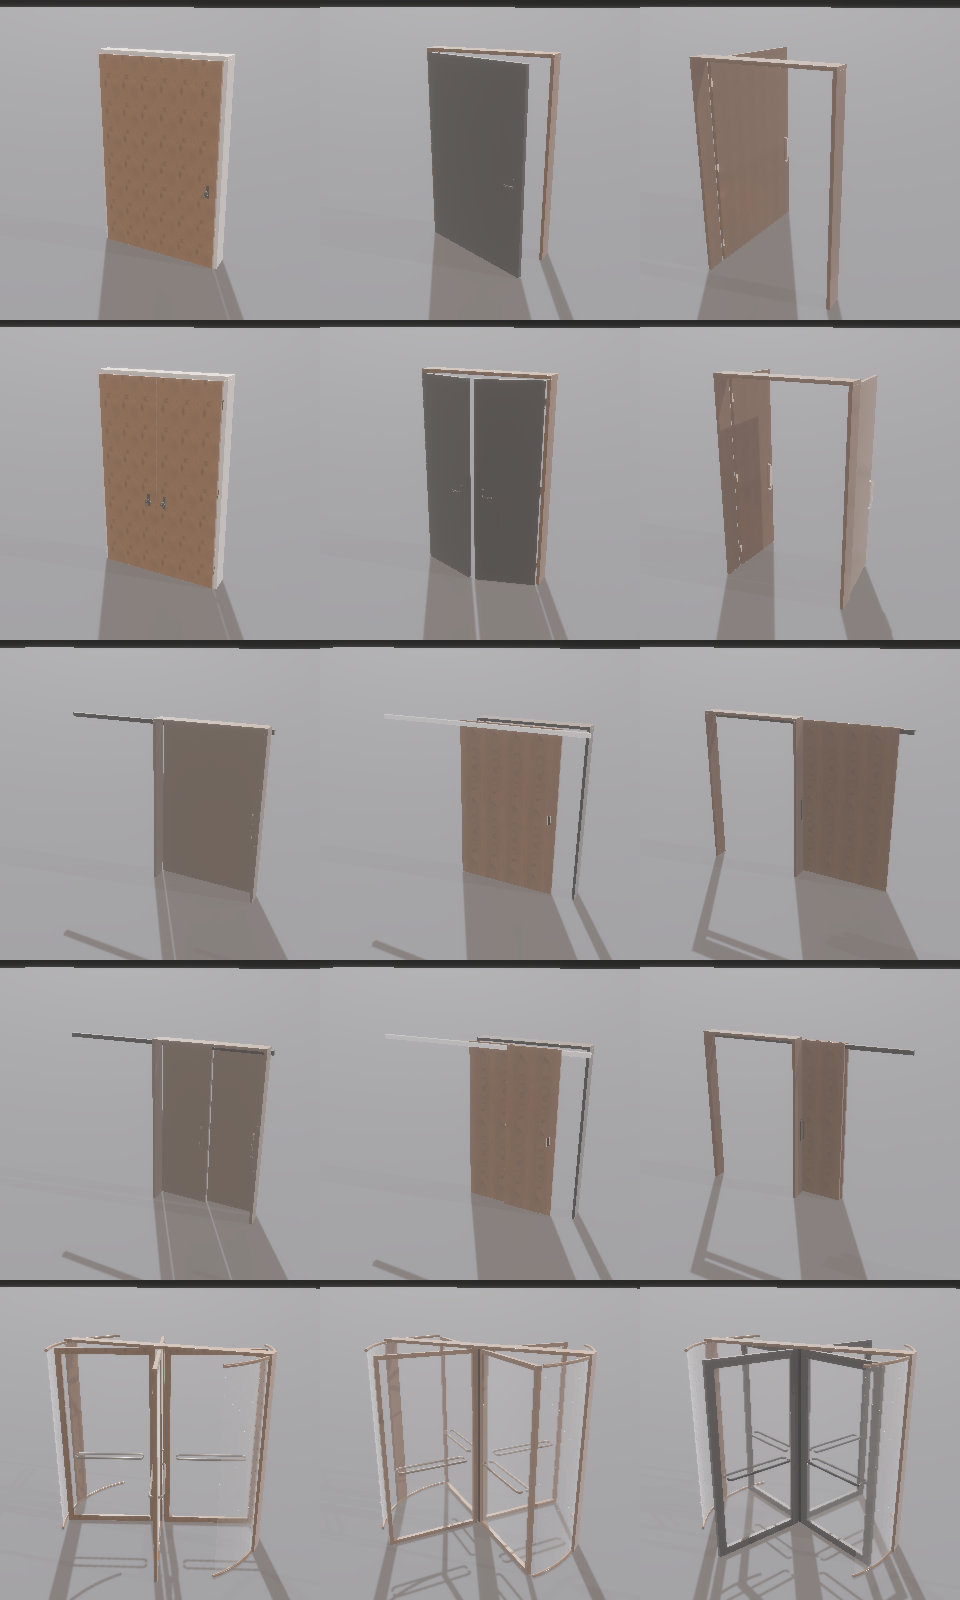
\includegraphics[width=.87\linewidth,height=.78\textheight,keepaspectratio]{doors_grid.png}\caption{Architectural door construction. Rows: hinged, paired, sliding, telescoping and revolving. The first four rows show sampled shut, ajar and open states; revolving rows show static rotor phases. Panel and finish parameters also vary.}\end{figure}
\begin{figure}[p]\centering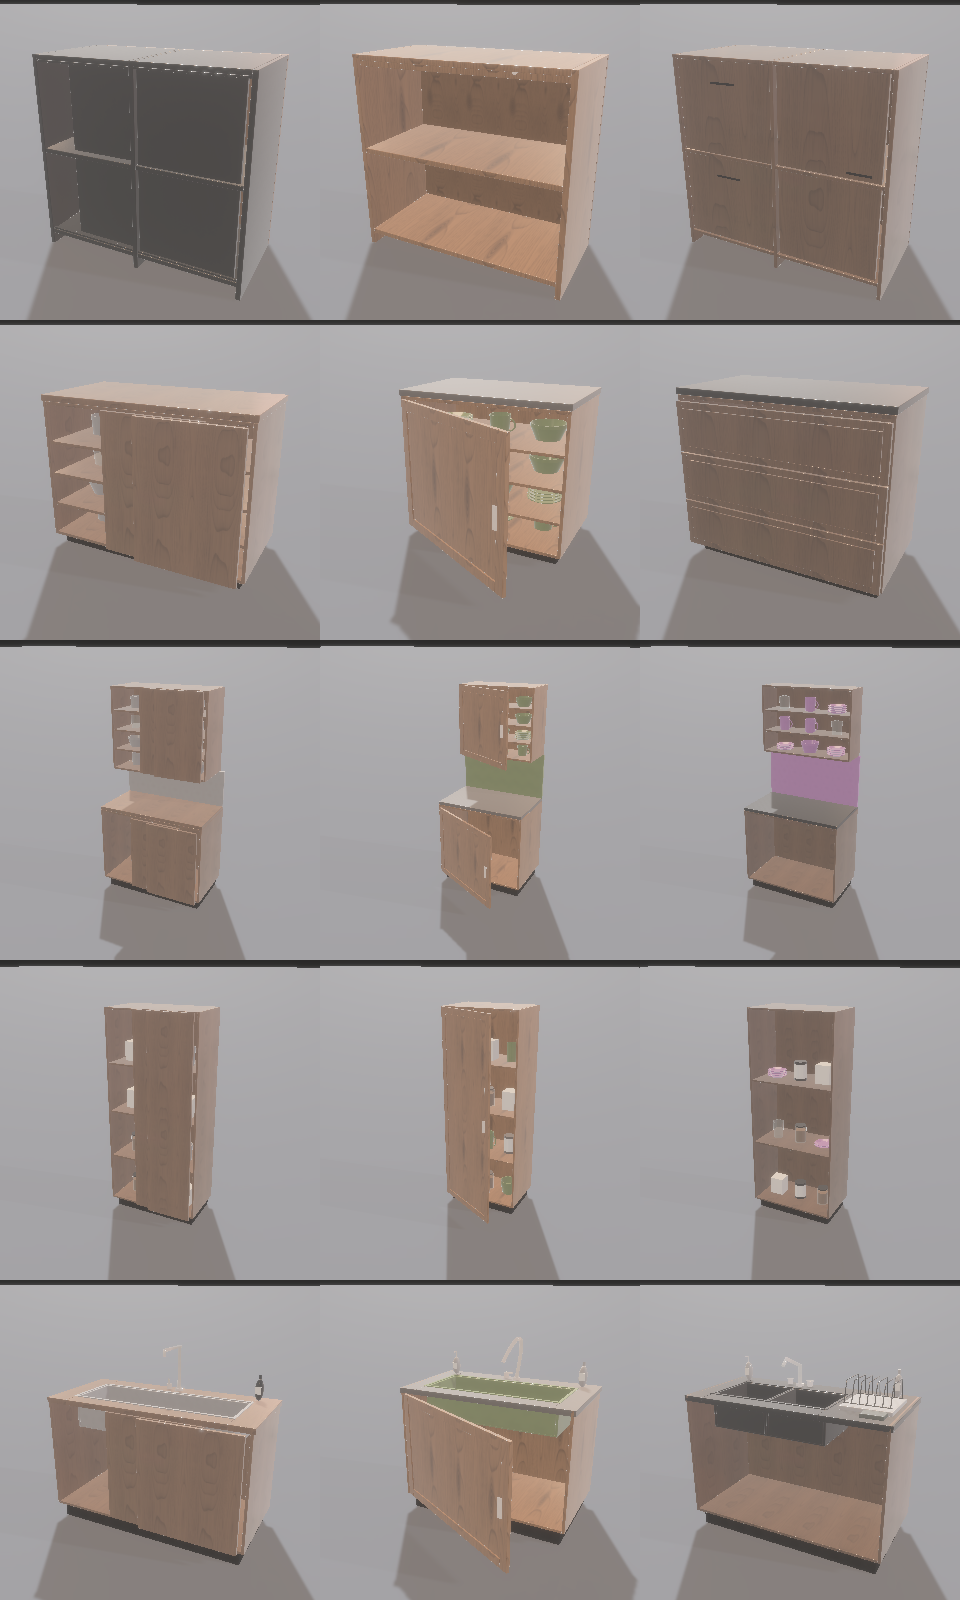
\includegraphics[width=.87\linewidth,height=.78\textheight,keepaspectratio]{cabinetry_grid.png}\caption{Cabinetry construction. Rows: office storage, counter base, base-and-overhead cupboard, pantry and sink base. Columns are prespecified seeds 0, 3 and 7, without visual filtering. All six examples and semantic/normal channels are available in the project-page category viewer.}\end{figure}

\end{document}
